\chapter{提案手法}
本研究では犬の行動推定のために,動画像・音声のマルチラベル分類を行った.
まず,入力となる動画から静止画のフレーム($F_t$)を取り出し,直後の$F_{t+1}$間とのオプティカルフロー画像($O_t$)を生成する.次に両画像から同じ構造の2つのネットワークを用いて特徴量の抽出を行う.
そして対応する音声($A_t$)からメル周波数ケプストラム係数($M_t$)を求め,前述とは異なる構造のネットワークを用いて($M_t$)から特徴量の抽出を行う.
最後にこれら2つあるいは3つの特徴量の組み合わせ毎に結合し,分類ネットワークでクラス分類を行う.
この際に,音声をフレームと同じサイズで切り出すと特徴が著しく失われるため入力音声には$F_t$の前後0.5秒ずつを用いた.動画あるいは音声から実際に犬の行動を推定する場合を想定し,現実的で取り扱いやすい時間としてこれを設定した.

分類はフレーム毎に行った.
\section{音声と画像を用いたSound based Two-stream network}
1つ目の提案手法として,音声を用いたTwo-stream networkを提案する.
既存のTwo-stream networkを改造し,静止画と音声からの動画分類の手法である.
Two-stream networkと違い音声を用いるため,これをSound based Two-stream networkと呼称する.
本研究ではこのネットワークをクラス分類ではなくマルチクラス推定に用いる.
%音声と静止画を用いたマルチクラス分類
%音声とoptical flow画像を用いたマルチクラス分類

\begin{figure}[htbp]
 \begin{center}
  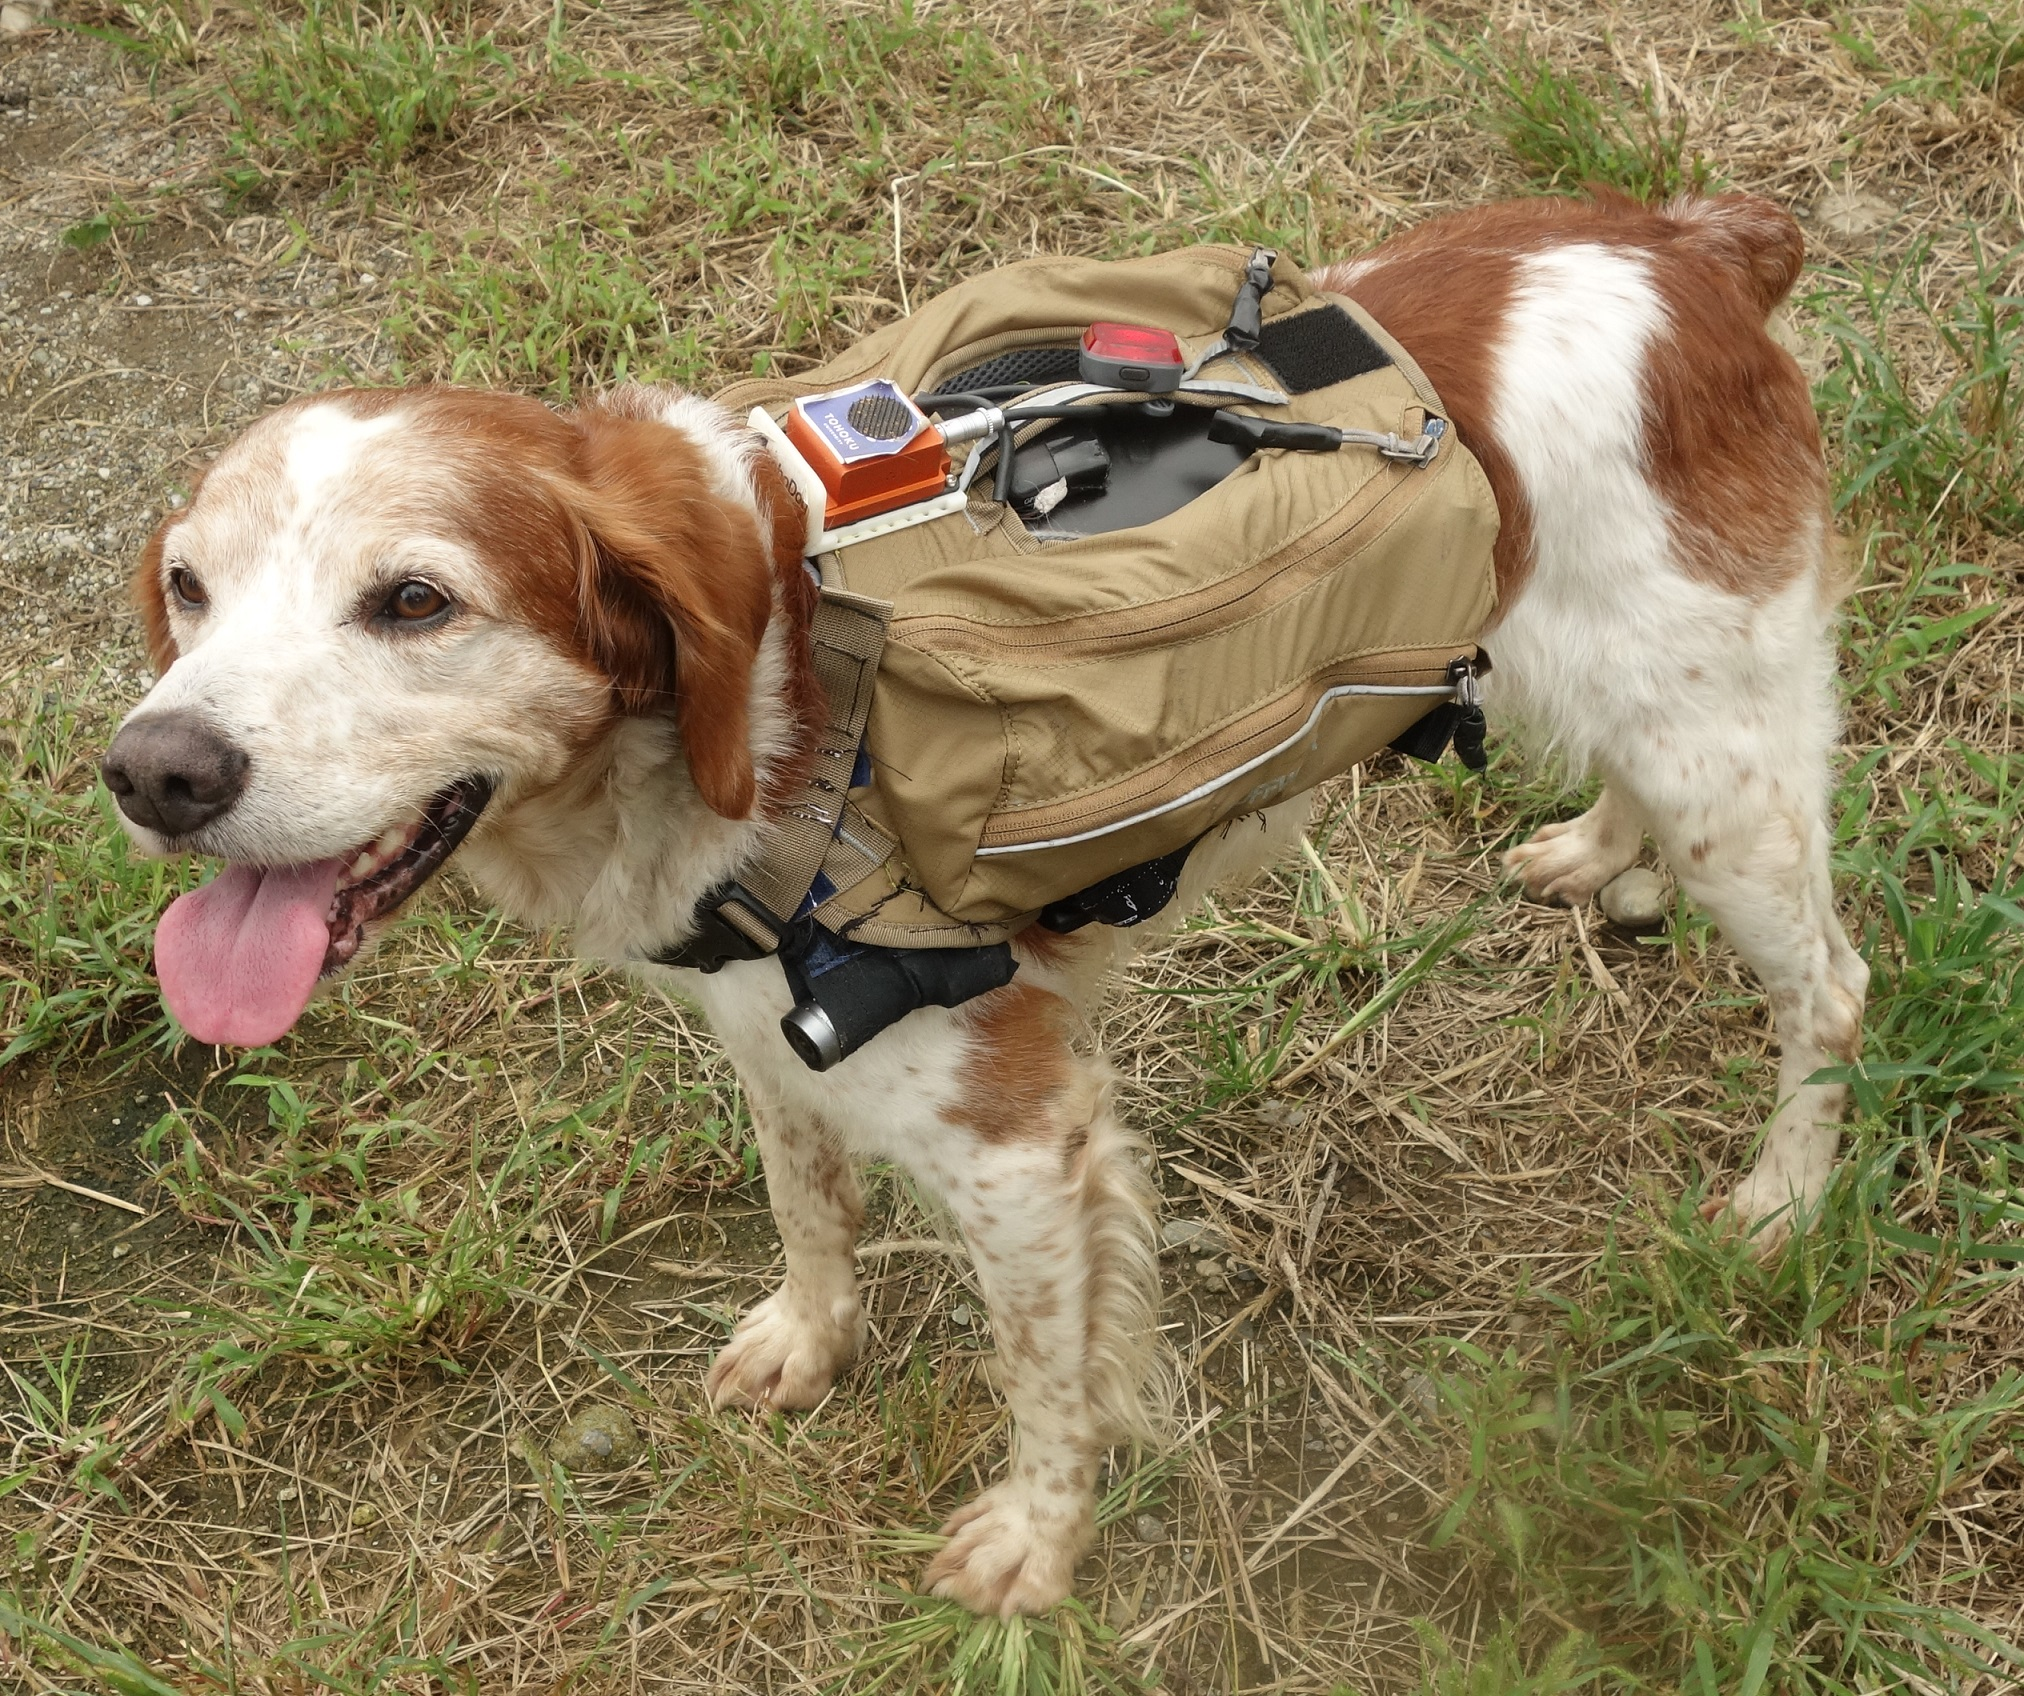
\includegraphics[width=9cm]{./Figures/cyberdog.eps}
  \caption{Sound convolutional network のアーキテクチャ}
  \label{sound-network}
 \end{center}
\end{figure}

\begin{figure}[htbp]
 \begin{center}
  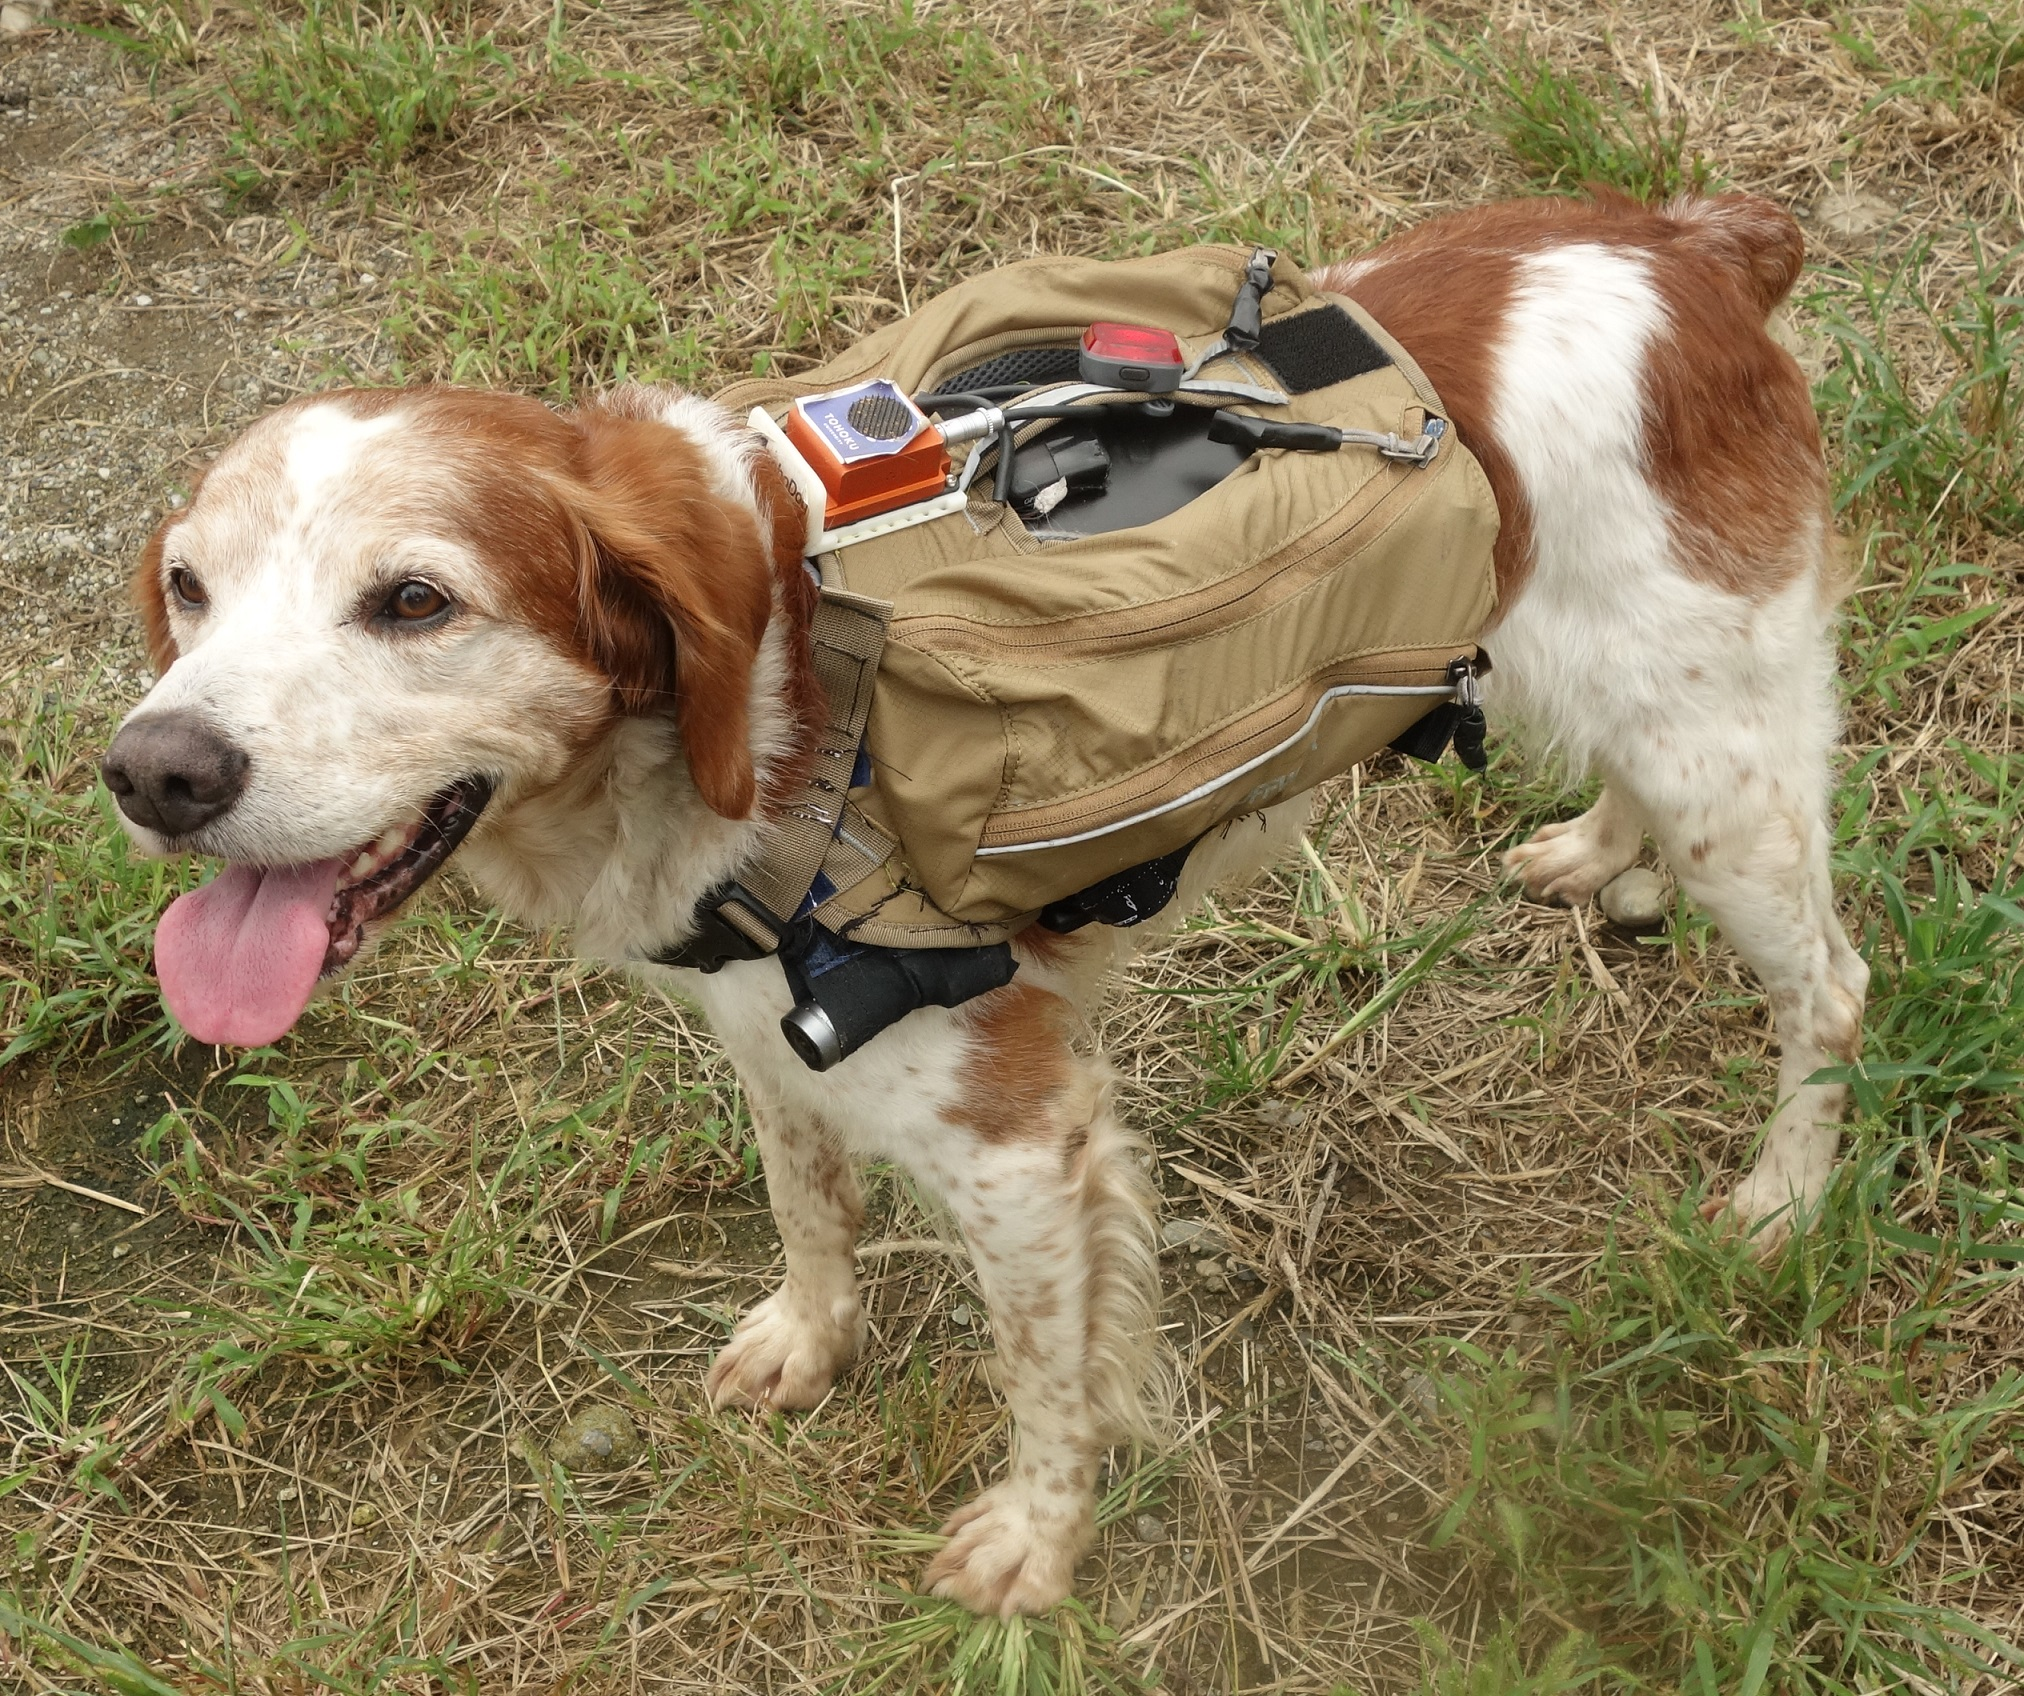
\includegraphics[width=9cm]{./Figures/cyberdog.eps}
  \caption{Sound based Two-stream のアーキテクチャ}
  \label{sound-two-stream}
 \end{center}
\end{figure}



\section{音声・静止画・optical flow画像を用いたSound based Three-stream network}

\begin{figure}[htbp]
 \begin{center}
  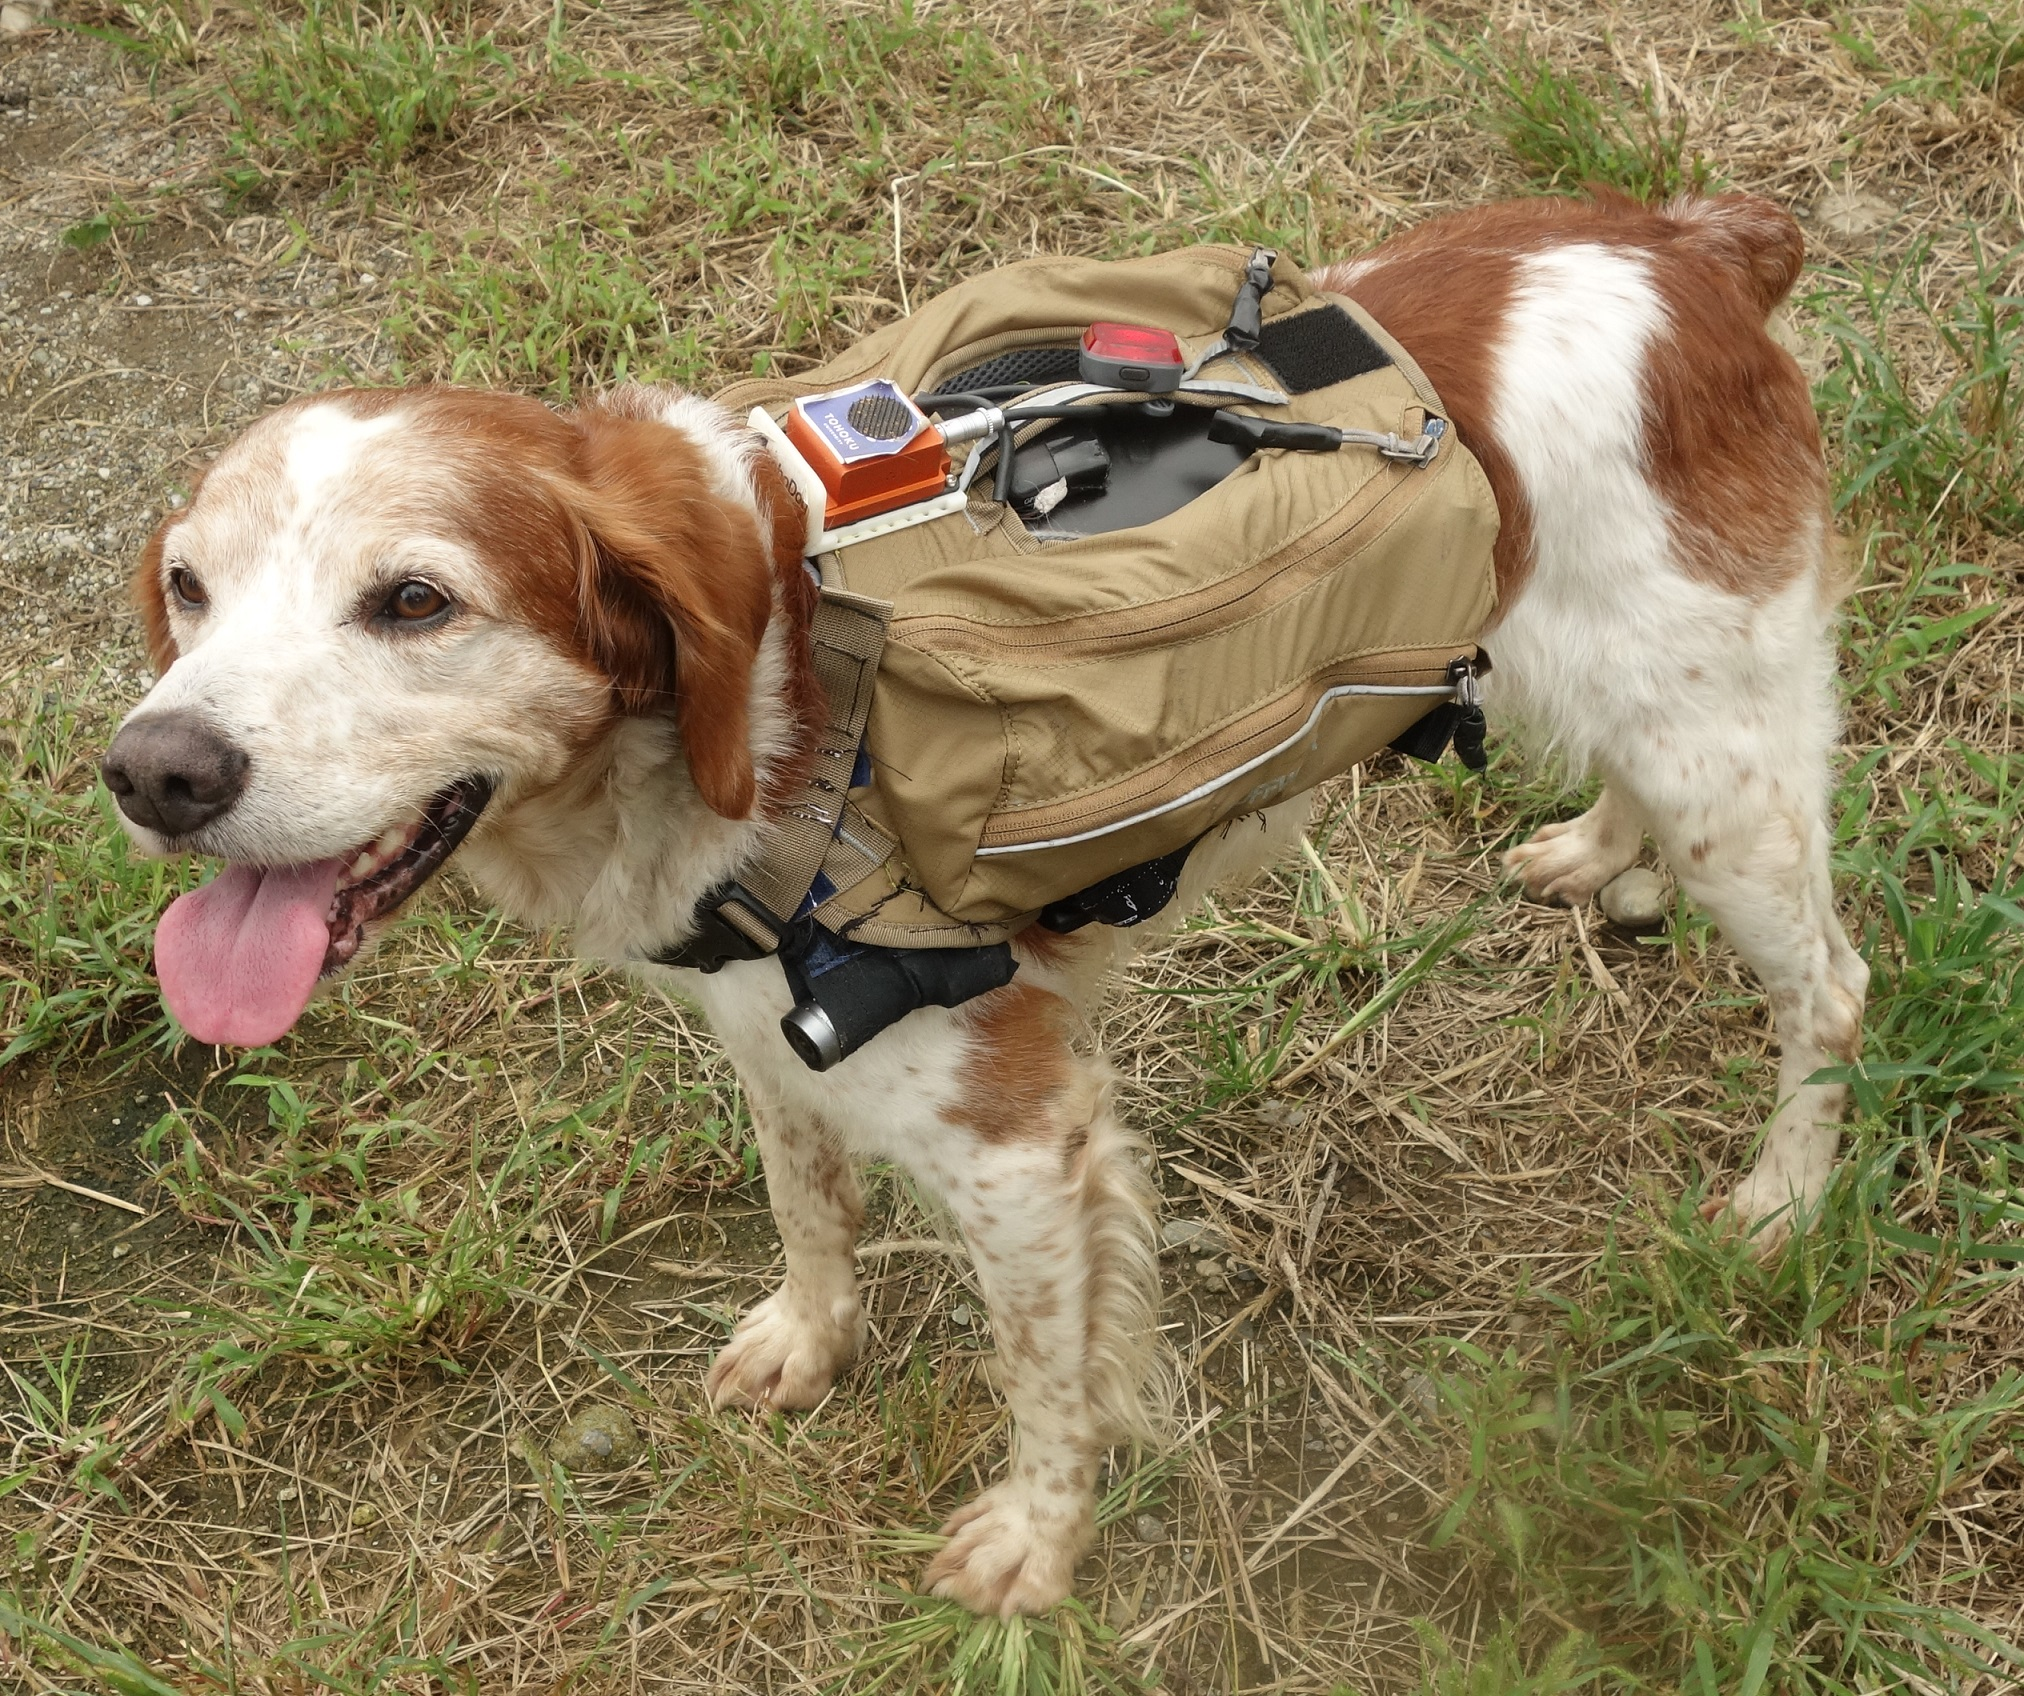
\includegraphics[width=9cm]{./Figures/cyberdog.eps}
  \caption{Sound based Three-stream (提案手法)のアーキテクチャ}
  \label{sound-three-stream}
 \end{center}
\end{figure}
